\documentclass{article}
\usepackage{analysistex}
\usepackage{tikz-cd}
\usepackage{wrapfig}
\usepackage{graphicx}
\usepackage{subcaption}
\newtheorem{theorem}{Theorem}
\newtheorem{prop}{Proposition}
\newtheorem*{note}{Note}
\newtheorem{problem}{Problem}
\newcommand{\grad}{\nabla}

\title{3D Surface Reconstruction using Geodesic Energy Minimization}
\author{Achyut Bharadwaj}
\date{Summer 2026}
\begin{document}

\section{Introduction}
The core aim of this project is to reconstruct a 3D surface from a single picture using information from geodesics on the surface. In particular, the focus is on reconstructing surfaces formed by ruled papers. In this case, the geodesics we use to extract information about the 3D embedding are the rulings: the straight lines printed on the paper, which appear curved in the two-dimensional image once the paper itself is curved in three dimensions. \\~\\
Consider a horizontally ruled paper curled in a cylindrical way along the vertical axis and towards the camera, with the camera placed at a height above the paper along its center. The resulting two-dimensional image appears as a straight horizontal line at the center, with the horizontal lines on either side of it curving increasingly sharply the farther they are from the center line (see Figure below). This particular curl and camera placement are chosen only to make the example concrete; neither the underlying mathematics nor the implementation depends on them. 
\begin{figure}[h]
  \centering
  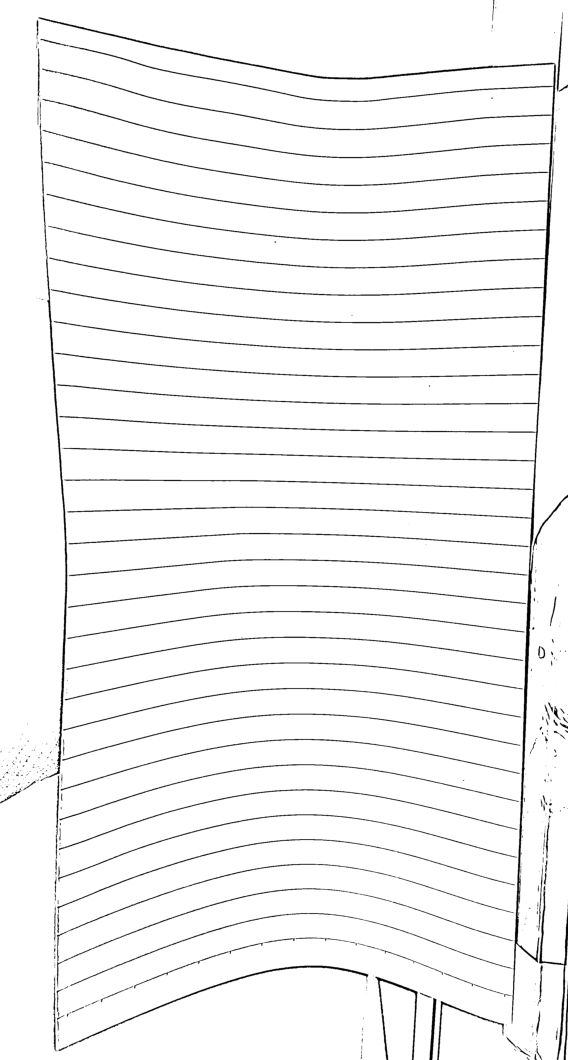
\includegraphics[width=0.3\textwidth]{example_curve.png}
  \label{fig:example_curve}
\end{figure}

The goal is to use the information contained in the lines' curvatures to recover the paper's original 3D embedding. Our method is as follows: we compute the curvature of each geodesic using the geometric form it assumes in the original 2D
image, integrate the square of this curvature along each geodesic, and sum the result across geodesics to obtain a net \emph{geodesic energy} of the flat image. We then compute a deformation of the flat surface and use a gradient descent algorithm to refine the computation to minimize the net geodesic energy. Theoretically, if the deformed surface matches the original 3D embedding, the energy must be exactly zero. \\~\\
The remaining sections detail the implementation and methodology in the order of application. Section~\ref{sec.trace} covers edge detection and curve tracing, which clean up the image and recover a dense cluster of points for each geodesic. Section~\ref{sec.fit} explains the conversion of each point cluster into an analytic curve whose derivatives—and hence curvature—are analytically computable; this same method generalizes to fitting surfaces to a cloud of points in three dimensions, which is utilized later. Section~\ref{sec.core} mathematically formalizes the geodesic energy functional and its computation for an arbitrary deformation of the image. Section~\ref{sec.gd} describes the gradient descent scheme used to minimize this energy. Finally, Section~\ref{sec.isgood} justifies why this energy-based approach is preferable to solving the boundary-value PDE directly, and Section~\ref{sec.lim} concludes with the current limitations of the implementation and directions for future improvement.

\section{Tracing Curves}\label{sec.trace}
This section details the detection of edges and the isolation of continuous curves from start to end. First, the raw grayscale image is binarized, coloring detected edges black and the background white via a process known as adaptive thresholding. \\~\\
The principle underlying adaptive thresholding involves iterating through all pixels in the grayscale image. At each pixel, the value is compared with the mean of a local neighborhood (e.g., a 30-pixel radius). If the value falls below the mean minus the standard deviation, the pixel is classified as black; otherwise, it remains white. This implementation is located in \verb|detector/edge_detector.py|. \\~\\
To mitigate susceptibility to noise, the grayscale image is first smoothed using a Gaussian blur low-pass filter. The transformation is defined by the following equation:
\[
  P_{\text{blur}}(x_0, y_0) = \sum_{(x, y) \in U}K(x-x_0, y-y_0) P(x, y)
\]
Here, $U$ is a small neighborhood of $(x_0, y_0)$, $P$ is the pixel value of the original image, and $P_{\text{blur}}$ is the pixel value of the filtered image. The term $K$ denotes the Gaussian Kernel, which is a normalized Gaussian distribution chosen appropriately for a given size of the neighborhood $U$. It suffices to choose a square or circle of fixed dimension around the origin and shift it appropriately to obtain $U$. \\~\\
This method is improved by using a weighted mean provided by the Gaussian Kernel rather than a naive unweighted mean. A fixed threshold parameter is often substituted for the standard deviation condition. For the remainder of the project, we use Gaussian blur followed by OpenCV's adaptive thresholding module, which implements this weighted approach. This is called directly in \verb|test_gd.py|. \\~\\
These preprocessing steps yield a clean binarized image with reduced noise and distinctly blackened rulings. See Figure \ref{fig:thresholding_pipeline} for results.
\begin{figure}[htbp]
    \centering
    \begin{subfigure}[b]{0.48\textwidth}
        \centering
        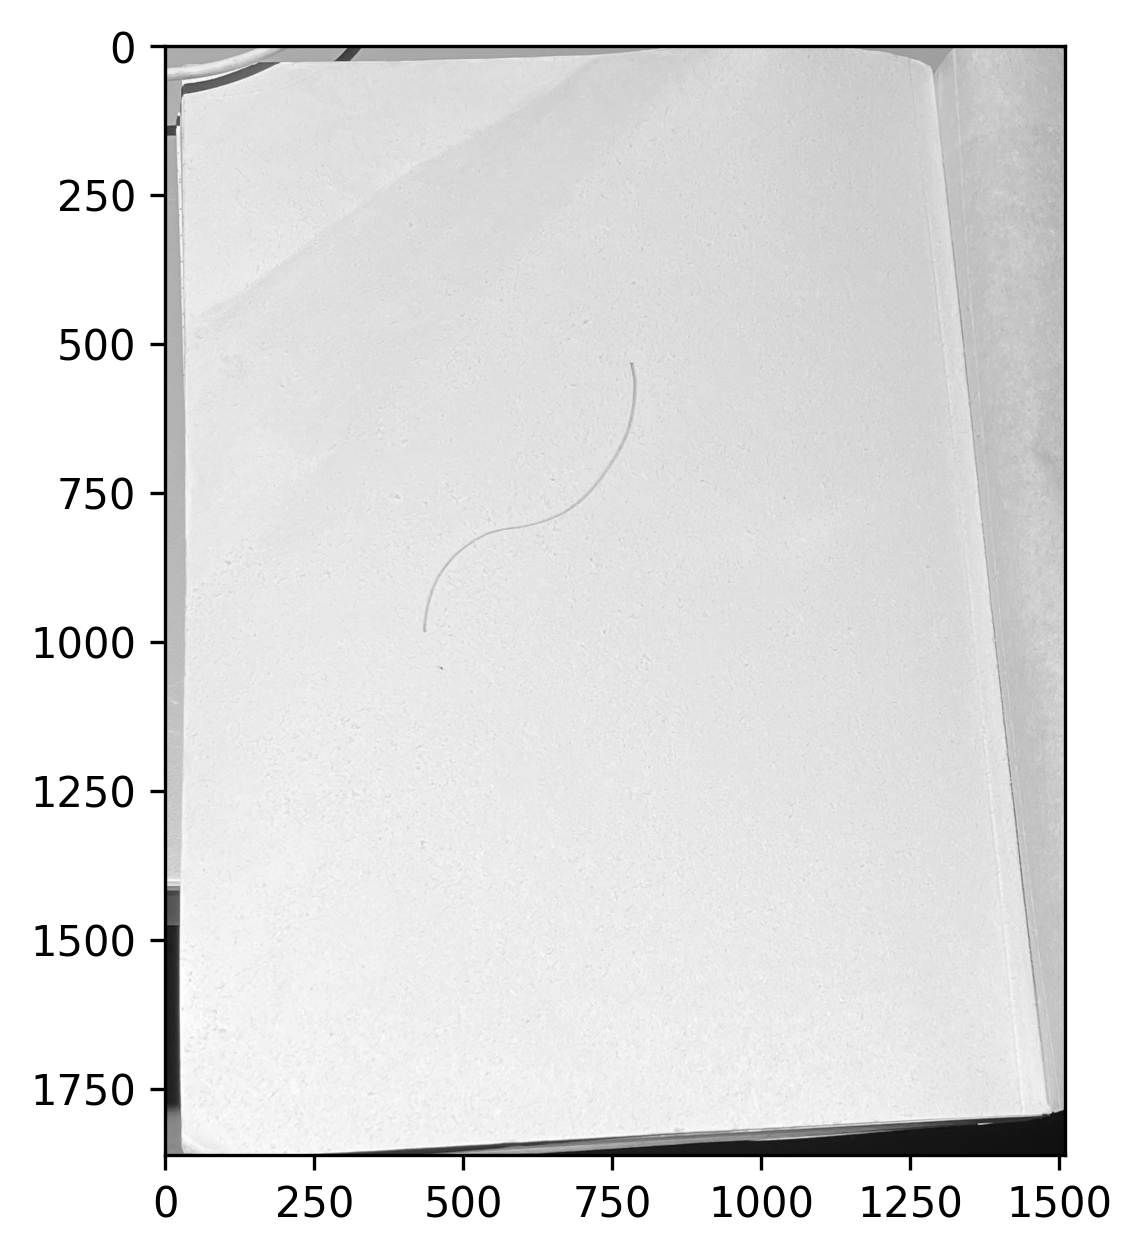
\includegraphics[width=\linewidth]{gray_img.png}
        \caption{Original grayscale image.}
        \label{fig:gray_img}
    \end{subfigure}
    \hfill
    \begin{subfigure}[b]{0.48\textwidth}
        \centering
        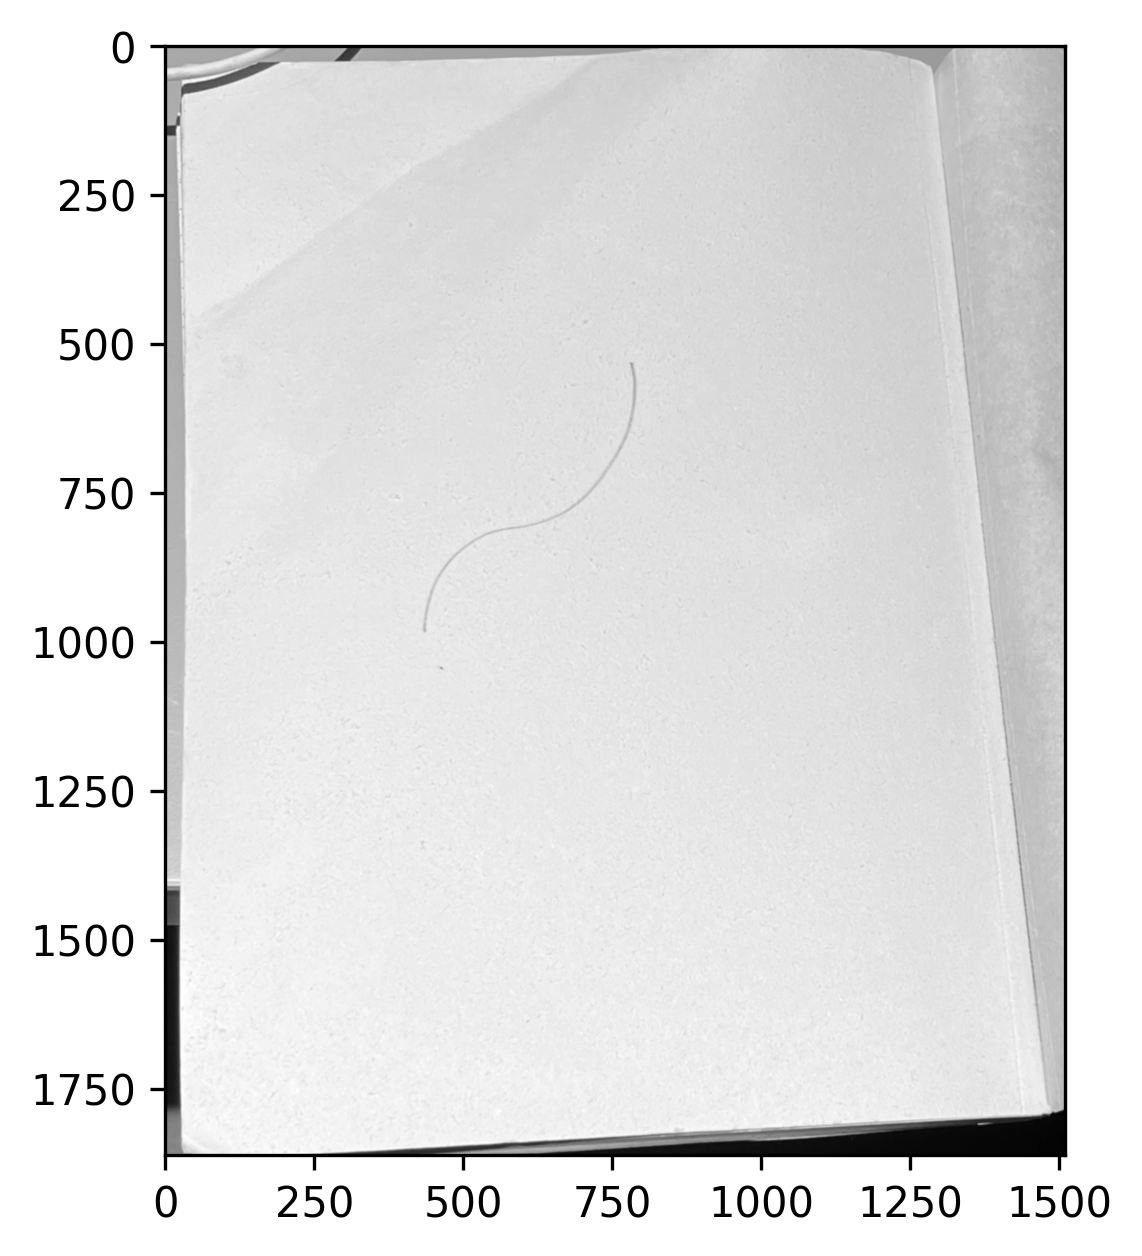
\includegraphics[width=\linewidth]{gaussian_blur.png}
        \caption{Grayscale image smoothed via Gaussian blur low-pass filter.}
        \label{fig:gaussian_blur}
    \end{subfigure}
    
    \vspace{0.8em}
    
    \begin{subfigure}[b]{0.48\textwidth}
        \centering
        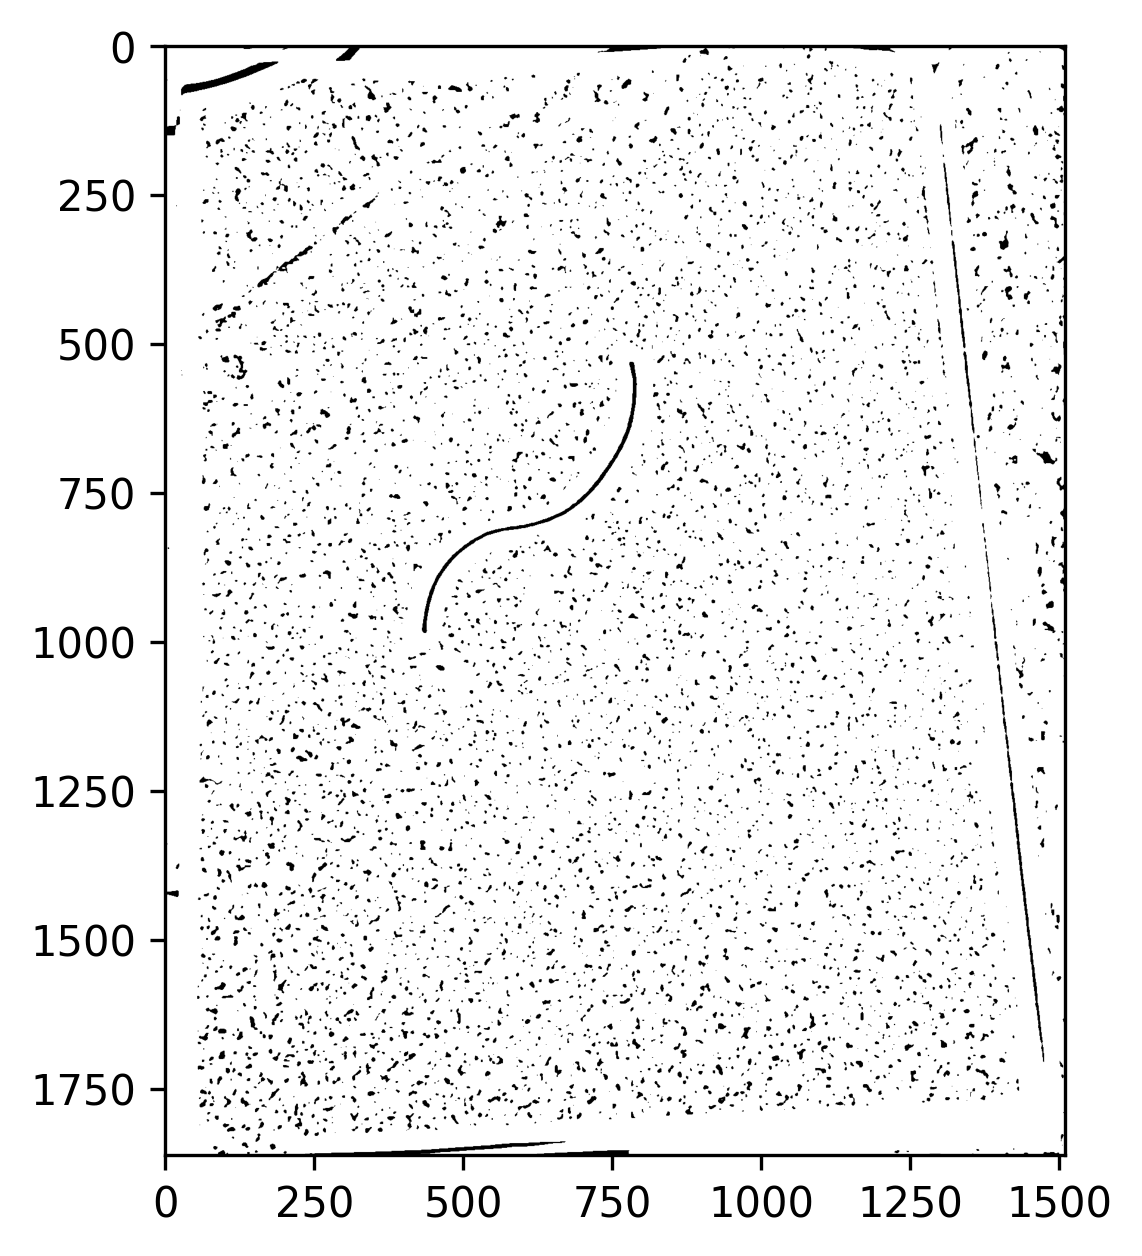
\includegraphics[width=\linewidth]{simple_clean.png}
        \caption{Adaptive thresholding using an unweighted local neighborhood mean.}
        \label{fig:simple_clean}
    \end{subfigure}
    \hfill
    \begin{subfigure}[b]{0.48\textwidth}
        \centering
        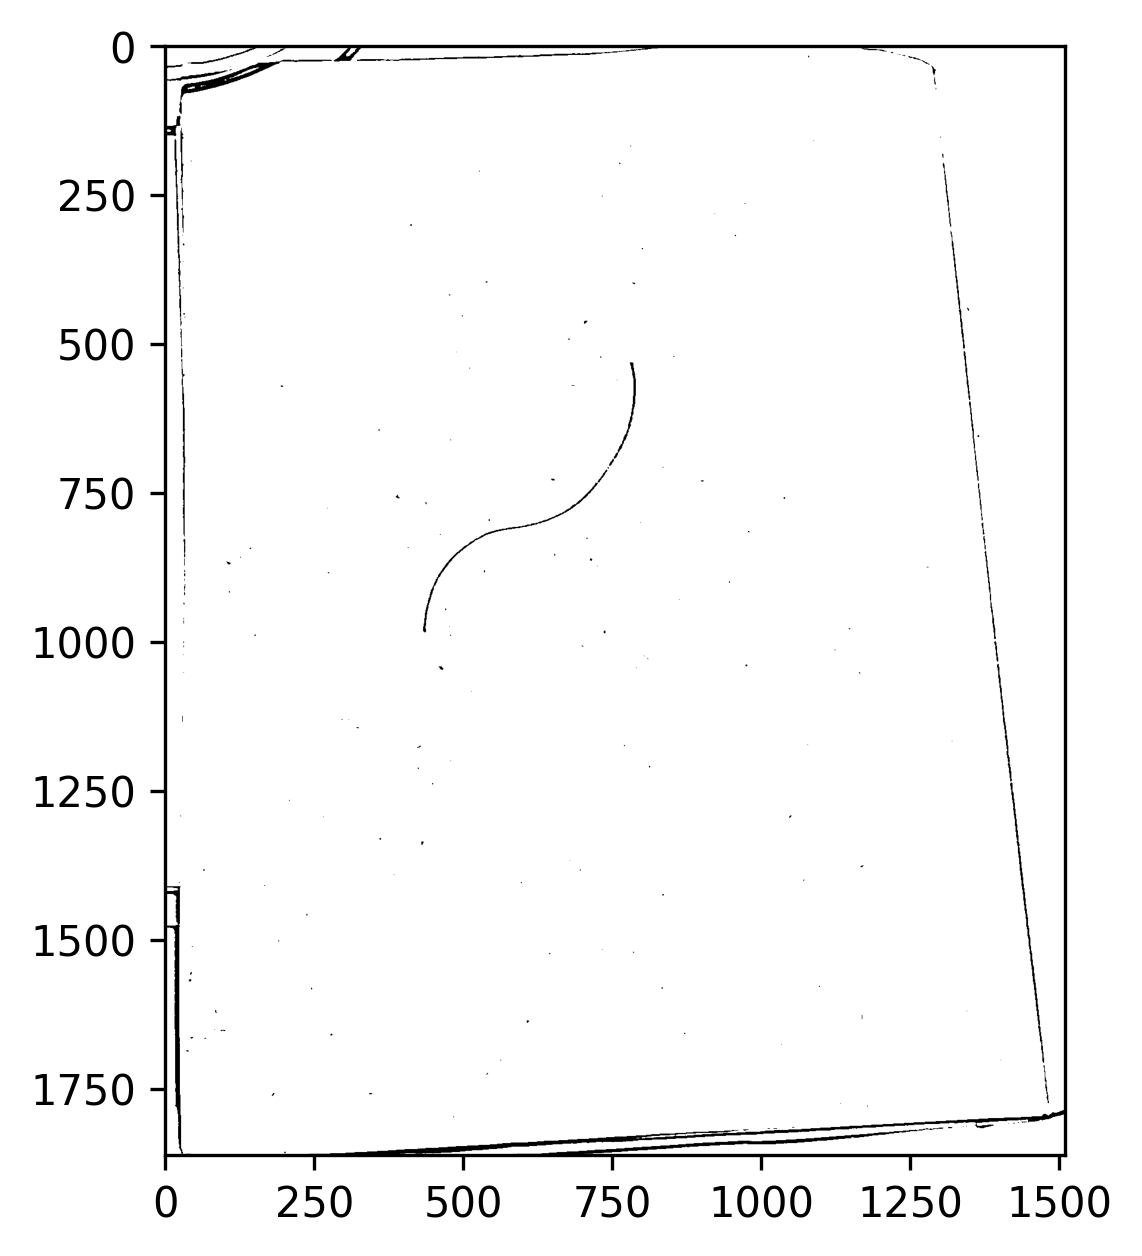
\includegraphics[width=\linewidth]{cv_clean.png}
        \caption{Adaptive Gaussian thresholding with weighted local neighborhood.}
        \label{fig:cv_clean}
    \end{subfigure}
    \caption{Comparison of image preprocessing stages: raw grayscale input, noise reduction via Gaussian blur, naive local mean thresholding, and OpenCV Gaussian adaptive thresholding.}
    \label{fig:thresholding_pipeline}
\end{figure}
The subsequent challenge involves tracing each ruling to output a list of discrete coordinate lines, enabling the isolation of individual geodesics for the remainder of the project. \\~\\
The tracing algorithm operates as follows: upon detecting a black pixel $p$, a $1\times n$ rectangle $Q$ (typically $2\times 5$) is fixed with one corner at $p$, representing a velocity vector. The algorithm computes the mean pixel value within $Q$, iteratively rotates $Q$ by a small angular increment (e.g., $5$ degrees), and records the mean pixel value at each step. The direction yielding the minimum mean pixel value, provided it falls below a specified threshold, is selected as the continuation of the curve. The opposite end of vector $Q$ becomes the new pivot $p$, and the process repeats until no further points satisfy the threshold condition. \\~\\
A naive execution of this algorithm often results in fragmented curves. This fragmentation persists even when maintaining a global \verb|visited| list to track traversed coordinates (which is necessary to prevent the program from entering an infinite loop during traversal). \\~\\
Fragmentation occurs when the iteration intersects the midpoint of a curve prior to identifying its endpoints, leading to the algorithm initiating a trace from the middle of a continuous line. To resolve this, conditions must be added to ensure that the algorithm never starts at a midpoint, and a \verb|sweep| variable is introduced to this end. Rather than finding a single global minimum across a full 360-degree rotation, the algorithm searches for local minima within discrete angular sectors defined by \verb|sweep|. Thus, $\theta$ is first iterated from $0$ to $\phi$ to find a minimum (if it meets the threshold requirement). The search proceeds to the next sector of $\phi$ degrees to find another local minimum, continuing the pattern. If multiple local minima are detected at the initiation of a trace, the coordinate is classified as a midpoint, and the trace is aborted. This ensures curves remain unbroken in non-intersecting geometries. \\

In the implementation, the mean is computed at 5-degree intervals. Local minima are evaluated using a sliding window of size $\phi/\theta$ on either side of each entry to determine whether it is a local minimum within that window.

The above approach is highly effective for most non-intersecting open curves. However, an additional condition terminates a curve if it exhibits sharp turns. This constraint excludes background noise or extraneous markings (e.g., text) outside the edge of the paper from being misidentified as geodesics.
\begin{figure}[htbp]
    \centering
    \begin{subfigure}[t]{0.48\textwidth}
        \centering
        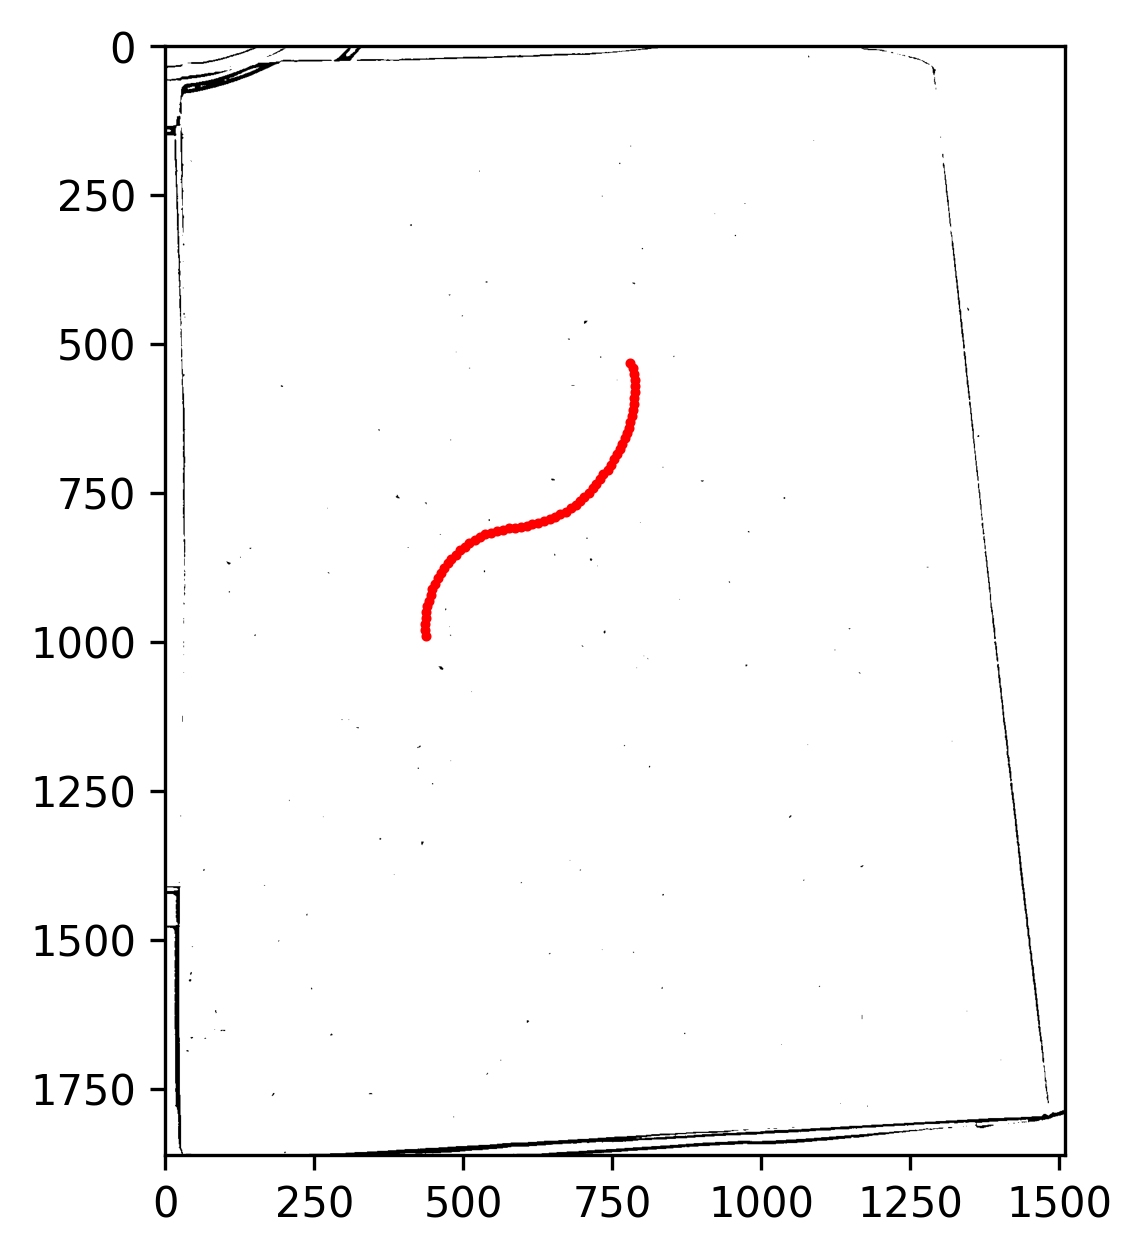
\includegraphics[width=\linewidth]{line_points.png}
        \caption{Extracted discrete pixel coordinates along a single isolated curve.}
        \label{fig:line_points}
    \end{subfigure}\hfill
    \begin{subfigure}[t]{0.48\textwidth}
        \centering
        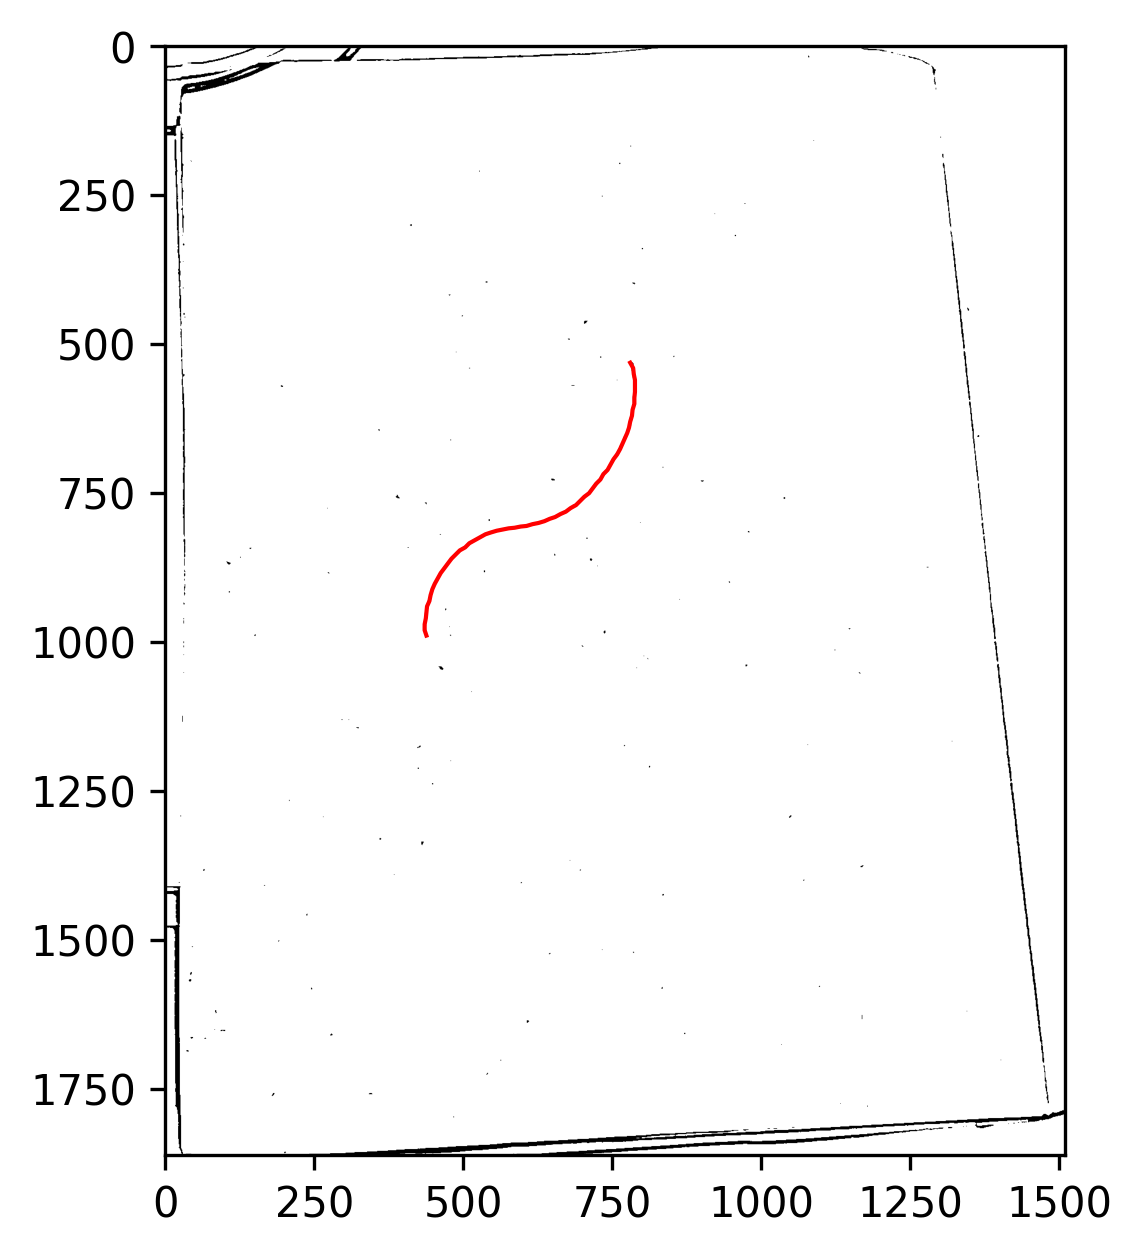
\includegraphics[width=\linewidth]{line_connected.png}
        \caption{Piecewise linear interpolation connecting the ordered sequence of extracted points.}
        \label{fig:line_connected}
    \end{subfigure}
    \caption{Tracing results for an isolated curve without the angle cutoff to prevent sharp turns. Overlaid on cleaned image.}
    \label{fig:line_extraction}
\end{figure}

\section{Fitting Curves using Splines}\label{sec.fit}
While the image processing isolates curves as discrete point sets, computing the acceleration at any given point requires an analytic representation. Subtracting adjacent velocity vectors derived from linear interpolation provides a crude approximation that fails to yield smooth acceleration values across all points. \\~\\
To resolve this, functions are fit to the discrete points $[(x_i, y_i)]$. Fitting a single global polynomial to an entire curve via least squares is impractical, as it is highly susceptible to underfitting and overfitting. However, the fit remains acceptable if restricted to a small subset of the full collection of points. By repeating this over multiple small neighborhoods, partitions of unity can naturally blend these local fit functions into a smooth global representation. \\~\\
The domain is divided into overlapping segments $U_i$. The dataset is restricted to $\{(x_j, y_j)\}_{x_j \in U_i}$, and a local function $f_i$ (typically quadratic) is fit to these points. A collection of smooth functions $\rho_i$ supported in $U_i$ (where $\rho_i(x) = 0$ for all $x \notin U_i$) is defined such that $\sum_{i} \rho_i = 1$ everywhere. The collection $(U_i, \rho_i)$ constitutes a partition of unity subordinate to the cover $U_i$. The global function is then $f(x) = \sum \rho_i(x) f_i(x)$. Since each $f_i$ is a local fit, $f(x)$ will resemble the global curve while guaranteeing infinite smoothness. \\~\\
Computing curvature requires the derivatives $f'(x)$ and $f''(x)$, which in turn necessitate the derivatives of $\rho_i(x)$. Once known, the computation is easily evaluated via the chain rule. Requiring $\rho_i$ to be strictly $C^\infty$ is computationally unfeasible; however, partitions of unity can be constructed such that $\rho_i \in C^k$, ensuring the first $k$ derivatives are easily computable. This methodology is detailed \href{https://personal.math.vt.edu/embree/math5466/lecture10.pdf}{here}. \\~\\
This approach assumes the dataset $\{(x_i, y_i)\}$ represents a standard function $y = f(x)$. Since rulings may be vertical rather than horizontal, a time domain $T = \{t_i\}$ is constructed to parameterize the dataset as $\{t_i, x_i, y_i\}$. Independent functions $x(t)$ and $y(t)$ are fit to obtain a full parameterization of the curve $\gamma$. Care must be taken in choosing the time domain to ensure two intervals of equal elapsed time contain approximately the same number of points, avoiding uneven fit quality. Fortunately, the curve tracing algorithm natively provides this uniformity: because a fixed-length vector was used to find successive points, consecutive points are equidistant in the plane. It therefore suffices to use total arclength to parametrize the dataset. This yields $x(t)$ and $y(t)$ along with their first two time derivatives, defining the curvature as $(x''(t), y''(t))$. Thus, derivatives are analytically computable at any continuous parameter $t$. \\~\\
\begin{figure}[htpb]
  \centering
  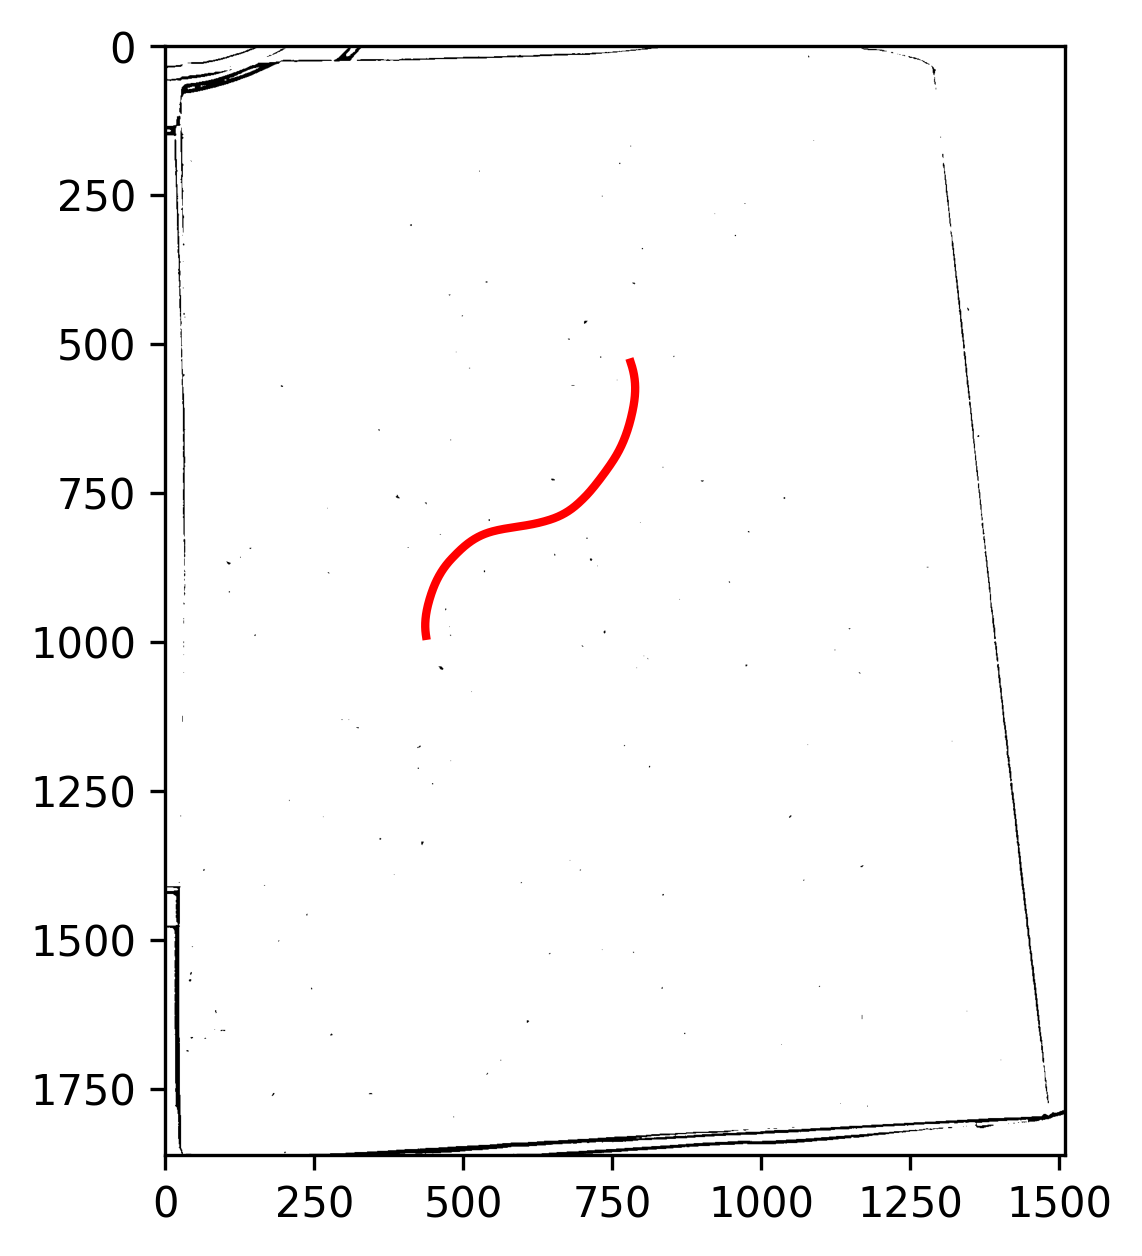
\includegraphics[width=0.5\textwidth]{curve_fit.png}
 \caption{Continuous curve reconstruction via partitions of unity.}
  \label{fig:curve_fit}
\end{figure}

Furthermore, this local fitting approach generalizes naturally to two dimensions (and higher). For a 3D point cloud $\{(x_i, y_i, z_i)\}$, the domain is divided into overlapping neighborhoods $U_i$ (e.g., rectangular bounds), local least squares polynomials are fit, and a subordinate partition of unity $\rho_i$ evaluates the global function and its derivatives. The 2D functions $\rho$ are easily constructed from the 1D functions $\rho_i$; if $\rho_j$ corresponds to the 1D bump function supported in $I_j$, the 2D formulation is defined as $U_{jk} = I_j \times I_k$ and $\rho_{jk} = \rho_j(x)\rho_k(y)$. \\~\\
In this project, a modified discrete approach is implemented. Rather than beginning with overlapping neighborhoods $U_i$ and fitting functions $f_i$ over all of $U_i$, the domain is partitioned into disjoint intervals of a fixed \verb|bin_size|. Denoting these disjoint partitions by $P_i$, we ensure that $P_i \subset U_i$. A function $f_i$ is fit over $P_i$ and applied across $U_i$ to generate the collection of functions $f_i$ and partitions $\rho_i$. \\~\\
See Figure \ref{fig:curve_fit} for a visual result of the curve fit. The interactive visualization of the fitted curves and derivative vectors can be evaluated by executing \verb|interface.py|. The program will request a cropped region, after which clicking on a curve and hovering over a point will display the continuous vectors.

\section{The Core Algorithm}\label{sec.core}
This section formalizes the core algorithmic approach. First, we establish the geometric information provided by a two-dimensional photograph of a curved piece of paper. \\~\\
Let $S \subset \R^3$ denote the target 3D surface, and assume the camera is positioned at the origin $0 \in \R^3$. The camera's image plane is defined as $P = \{(x, y, f) \colon x, y \in \R\}$, where $f$ is the focal length. The captured image $Q \subset P$ contains points that uniquely correspond to points on $S$ via spatial scaling (assuming full visibility of $S$). This projective correspondence preserves information: the pixel intensity at $(x, y, f) \in Q$ exactly equals the light intensity at $\lambda(x, y, f) \in S$, where $\lambda$ is the required scaling factor. \\~\\
Consequently, the image yields a subset $Q$ of coordinates $(x, y, f)$, and the objective is to determine a deformation of $Q$ that recovers $S$. We must ensure that the deformation continues to preserve the projective correspondence derived from scaling. More precisely, we seek a function $\phi \from Q \to \R^3$ subject to the constraint $\phi(x) = \lambda_x x$ for some $\lambda_x\neq 0 \in \R$, such that $\phi(Q) = S$. Equivalently, the goal is to define a scalar function $\rho \from Q \to \R$ such that the deformed surface $S_\rho \defeq \{\rho(x) x \colon x \in Q\}$ matches $S$. \\~\\
While this formulation is mathematically precise, it requires additional constraints to recover $S$, as the true surface geometry is unknown. This is where the rulings provide necessary geometric constraints. In 3D space, $S$ is a surface, and the rulings are geodesics on $S$. However, when a picture of $S$ is taken, the curves are pointwise transferred to the image $Q$, yet they are no longer geodesics on the flat image plane. To be precise, let $\eta \from [0, 1] \to S$ parameterize a geodesic on $S$. For simplicity, assume that $\eta$ has a constant speed of $1$ (in practice, this assumption is abandoned to make computations work out), and until explicitly stated, assume all curves have constant speed $1$. The curve $\eta$ has no acceleration outside of the surface's own bending (this is the definition of a geodesic). Thus:
\[
  \int_0^T \abs{[\ddot \eta(t)]^T}^2 dt = 0
\]
Conversely, for the corresponding projected curve $\gamma(t)$ in $Q$, this integral is strictly non-zero. Here, $\ddot \gamma(t)^T$ denotes the projection of the acceleration vector onto the tangent space at the point $\gamma(t)$. The procedure is therefore established: we search for $\rho \from Q \to \R$ to minimize the tangential acceleration of the lifted curve $\gamma_\rho(t) \defeq \rho(\gamma(t)) \gamma(t)$ on the deformed surface $S_\rho$:
\[
  E_\gamma[\rho] = \int_0^{T_\rho} \abs{[\ddot \gamma_\rho(t)]^t}^2 dt = \int_0^{T_\rho} \abs{\left[\frac{d^2}{dt^2}(\rho(\gamma(t))\gamma(t))\right]^T}^2 dt = 0
\]
While multiple incorrect surfaces might satisfy $E_\gamma[\rho] = 0$ for a single curve, minimizing this functional across a dense set of different $\gamma$ curves converges on the true surface geometry. While the four edges of a rectangular paper theoretically suffice to uniquely determine the original embedding (up to scaling)—prompting the question of why an energy-based approach is necessary—computing this exact embedding requires solving a PDE with boundary conditions derived from those edges. Small, inevitable observational errors in detecting the boundary can cause the PDE to yield no solutions or infinitely many solutions. In simple terms, while an exact analytical computation is possible, the energy minimization approach is vastly more robust to real-world measurement error. The mathematically inclined reader may refer to Section \ref{sec.isgood} for a deeper justification of the energy functional. \\

To this end, we define the total geodesic energy functional $E \from C^\infty(Q) \to \R$ as $\rho \mapsto \sum_\gamma E_\gamma[\rho]$. We assume $\rho$ is smooth since $S$ must be smooth. Because strictly achieving $E[\rho] = 0$ is unachievable in practice due to discretization and noise, the core method to recover $S$ relies on minimizing $E[\rho]$ using gradient descent. \\

The remainder of this section focuses on computing the energy more explicitly, which assumes familiarity with differential geometry. For readers experienced in this field, the tangential acceleration that we want to compute is exactly the geodesic curvature $\kappa_g$ of $\gamma_\rho$, which is explicitly given by the standard formula:
\[
  \kappa_g = \frac{(N \times \dot\gamma_\rho)\cdot \ddot\gamma_\rho}{\abs{\dot \gamma_\rho}^3}
\]
Squaring and integrating this term (after applying a change of variables to account for non-uniform speed) directly yields an explicit expression for the energy:
\[
  E_\gamma[\rho] = \int_0^T \abs{[\ddot \gamma_\rho(t)]^T}^2 dt = \int_0^1\frac{\abs{N(\gamma_\rho(s)) \cdot (\dot \gamma_\rho(s)\times \ddot \gamma_\rho(s))}^2}{\abs{\dot\gamma(s)}^5}ds
\]
The normal can be computed using $\rho$ itself as the parametrization, and all derivatives are evaluated using the chain rule. The explicit details of this computation are provided below for readers less familiar with these derivations. \\

Assuming the derivatives of $\gamma$ with respect to $t$ are accurately computed (as established in Section \ref{sec.fit}), the derivatives of $\rho$ with respect to $x$ and $y$ can be computed similarly. Applying the chain rule to compute $\rho'(t)$ and $\rho''(t)$ directly yields $\ddot \gamma_\rho(t)$. We must then compute the tangential projection $\ddot \gamma(t)^T = X(p)^T$, where $p = \gamma_\rho(t)$, and factor the arbitrary speed into the equations. \\~\\
Fix a point $p \in S_\rho$ and suppose that $X$ is a vector in $\R^3$ with basepoint $p$. The vector $X$ decomposes orthogonally as $X = X^T + (X\cdot N) N$, where $N$ is the normal vector at $p$. Thus, computing the normal $N(p)$ of $S_\rho$ is required. This is achieved by constructing a parametrization for $S_\rho$ around $p$ defined by $\varphi(x, y) \defeq \rho(x, y, f) (x, y, f) \in S_\rho$. Note that when $p = \gamma_\rho(t)$, the coordinates map to $(x_0, y_0, f) = \gamma(t)$. 
The tangent plane $T_p S_\rho$ is spanned by $\{\del_x \varphi (p), \del_y \varphi(p)\}$. The normal $N(\gamma_\rho(t))$ is therefore:
\[
  N(\gamma_\rho(s)) = \frac{\del_x \varphi(x_0, y_0) \times \del_y \varphi(x_0, y_0)}{\norm{\del_x \varphi(x_0, y_0) \times \del_y \varphi(x_0, y_0)}}
\]
where $(x_0, y_0, f) = \gamma(s)$. The partial derivatives are computed via the product rule:
\[
  \del_x \varphi(x_0, y_0) = (\del_x \rho(x_0, y_0) x_0 + \rho(x_0, y_0), \del_x \rho(x_0, y_0) y_0, \del_x \rho(x_0, y_0)f)
\]
Because the parameterization speed is not necessarily constant, a further cross product with the velocity vector $\dot \gamma_\rho(t)$ must be taken to ensure that any nonzero tangential acceleration remains strictly aligned with the direction of the curve (representing scalar speeding up or slowing down). Accounting for this, we have $\ddot \gamma_\rho(t)^T = N(\gamma_\rho(t)) \cdot (\dot \gamma_\rho(t)\times \ddot \gamma_\rho(t))$. The remainder of the calculations depend explicitly on $\rho$ and $\gamma$, detailed in the \verb|evaluate_penalties| method of \verb|detector/energy.py|. \\~\\
Finally, because $\gamma(s)$ is parameterized by an arbitrary variable $s \in [0, 1]$ rather than its true arclength parameter $t$, the change of variables $dt = \abs {\dot \gamma_\rho(t)}ds$ is applied, yielding:
\[
  E_\gamma[\rho] = \int_0^T \abs{[\ddot \gamma_\rho(t)]^T}^2 dt = \int_0^1\frac{\abs{N(\gamma_\rho(s)) \cdot (\dot \gamma_\rho(s)\times \ddot \gamma_\rho(s))}^2}{\abs{\dot\gamma(s)}^5}ds
\]
Differentiating $\gamma_\rho(s)$ with respect to $s$ introduces a factor of $1/\abs{\dot \gamma_\rho(s)}$ at each step. Differentiating three times in the numerator and squaring contributes a factor of $\abs{\dot \gamma_\rho(s)}^{-6}$, which, when multiplied by $\abs{\dot \gamma_\rho(s)}$ from the change of variables, results in the final $\abs{\dot \gamma(s)}^{-5}$ scaling term. \\~\\
In addition to the core geodesic energy computed above, the \verb|evaluate_penalties| method includes optional penalization parameters for high mean/Gaussian curvature and arclength variance. These are currently set to $0$ but can be fine-tuned to constrain the geometry, though the implementation primarily relies on the geodesic energy.

\section{Gradient Descent}\label{sec.gd}
The final stage of the algorithm utilizes gradient descent to find a minimizer $\rho$ for the functional $E$. While gradient descent is standard for functions $f \from \R^N \to \R$ over finite-dimensional spaces, the energy functional operates over the infinite-dimensional space $C^\infty(Q)$. The practical resolution is discrete approximation. The domain $Q$ is sampled across a uniform grid $D = \{(u_i, v_i)\colon i = 1, 2, \dots, N\}$. The continuous function $\rho$ is represented by a finite vector $\vect x \in \R^N$ where $x_i = \rho(u_i, v_i)$, effectively reducing the objective to $E \from \R^N \to \R$. \\~\\
The gradient descent algorithm proceeds as follows:
\begin{itemize}
  \item Initialize $\vect x_0 = (1, 1, \dots, 1)$, corresponding to the discrete representation of a flat plane $\rho(x, y, f) = 1$ for all $(x, y, f) \in Q$.
  \item Fit a smooth global quadratic surface to the coordinates $(u_i, v_i, x_i)$ to estimate continuous partial derivatives $\rho_u$, $\rho_v$, $\rho_{uv}$, $\rho_{uu}$, and $\rho_{vv}$. This utilizes the methodology from Section \ref{sec.fit} with a sufficiently large \verb|bin_size| to obtain a global fit. See Section \ref{sec.lim} for an explanation of why a global fit is necessary instead of localized bump functions.
  \item Iterate through the detected curves and compute $E_\gamma[\rho]$ using the fitted surface $\rho$ and its analytic derivatives.
  \item Sum the individual curve energies to obtain the total energy and compute the gradient $\grad E(\vect x)$ via automatic differentiation.
\end{itemize}
Reverse-mode automatic differentiation allows for the computation of derivatives for any algorithmically defined function. In this implementation, the input is $\vect x$ and the function $E(\vect x)$ encompasses both the numerical integration and the surface fitting operations. PyTorch is utilized to perform this autodifferentiation. The discrete surface is iteratively updated via standard gradient descent: $\vect x_{n+1} = \vect x_n - \eta_n\grad E(\vect x_n)$. The iteration terminates after a fixed number of steps or when the gradient magnitude falls below a specified threshold (configured in \verb|test_gd.py|). \\~\\
The standard approach is implemented in \verb|detector/gradient_descent.py| via \verb|run_vanilla_descent|. Additionally, gradient descent with momentum is supported via \verb|run_adam_descent|, leveraging PyTorch's Adam optimizer to accelerate convergence. \\

\begin{figure}[htbp]
    \centering
    \begin{subfigure}[t]{0.48\textwidth}
        \centering
        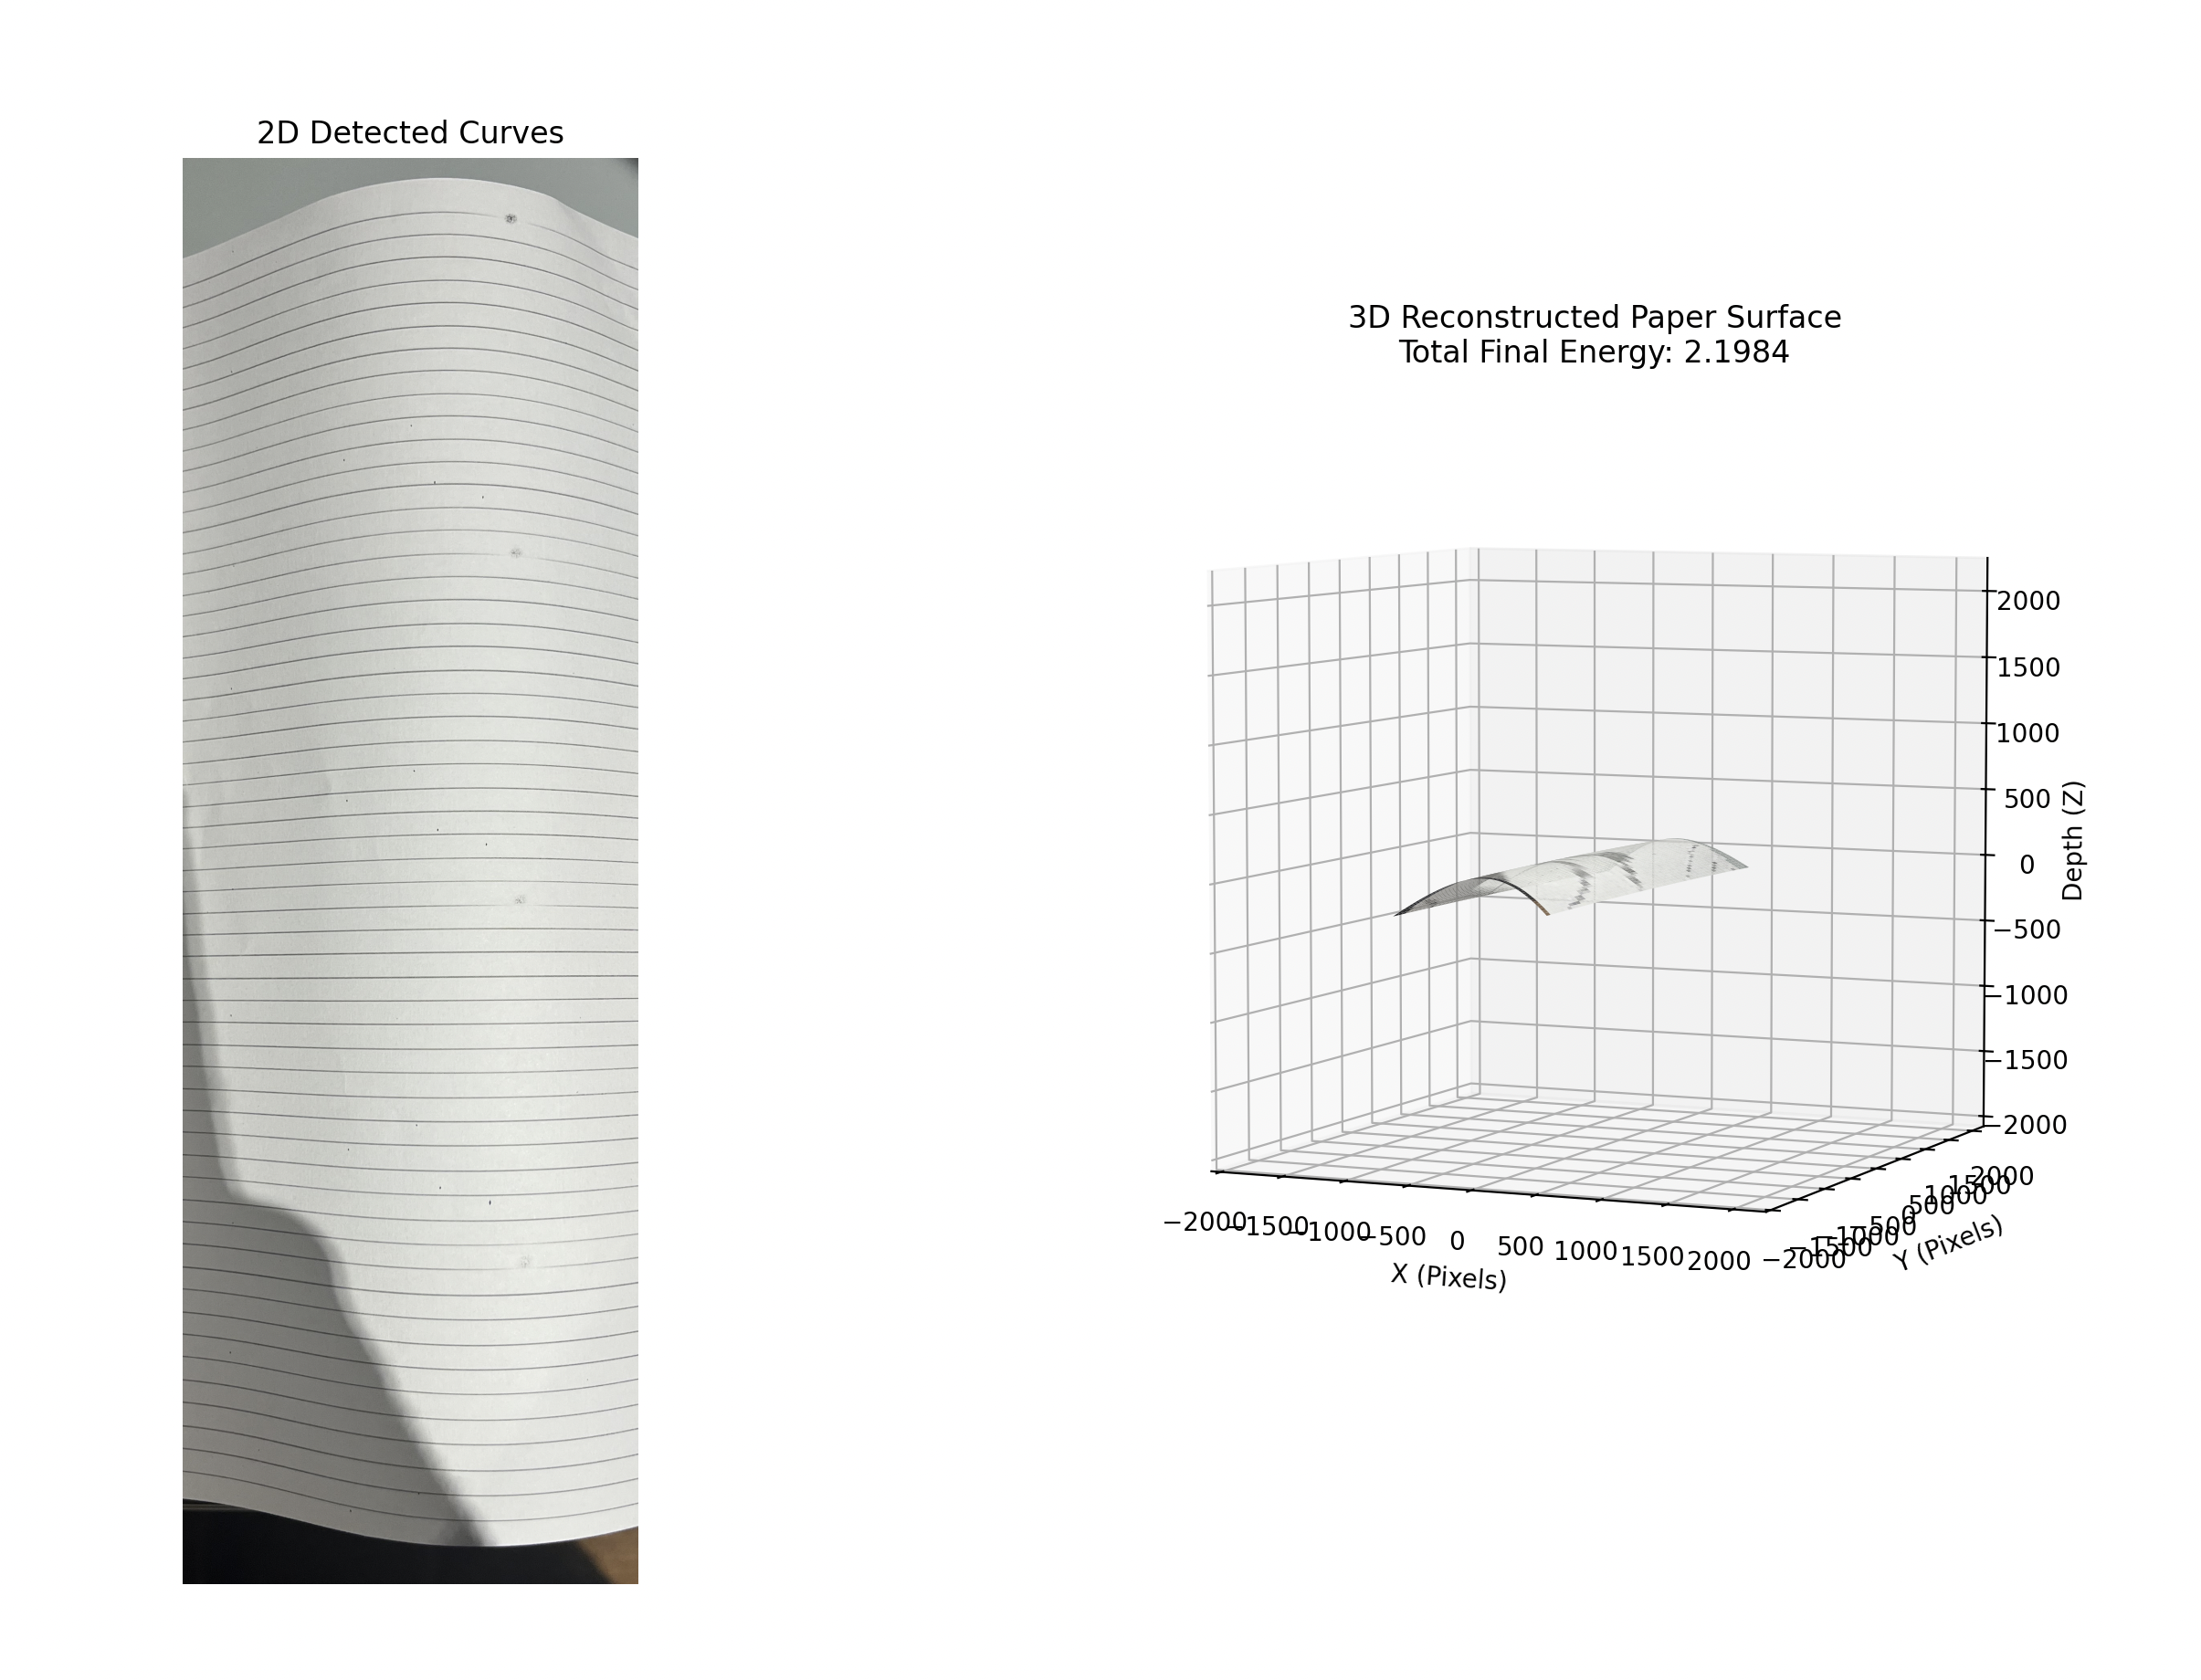
\includegraphics[width=\linewidth,height=0.34\textheight,keepaspectratio]{upcurve.png}
        \caption{Convex deformation (surface curving toward camera).}
        \label{fig:upcurve}
    \end{subfigure}\hfill
    \begin{subfigure}[t]{0.48\textwidth}
        \centering
        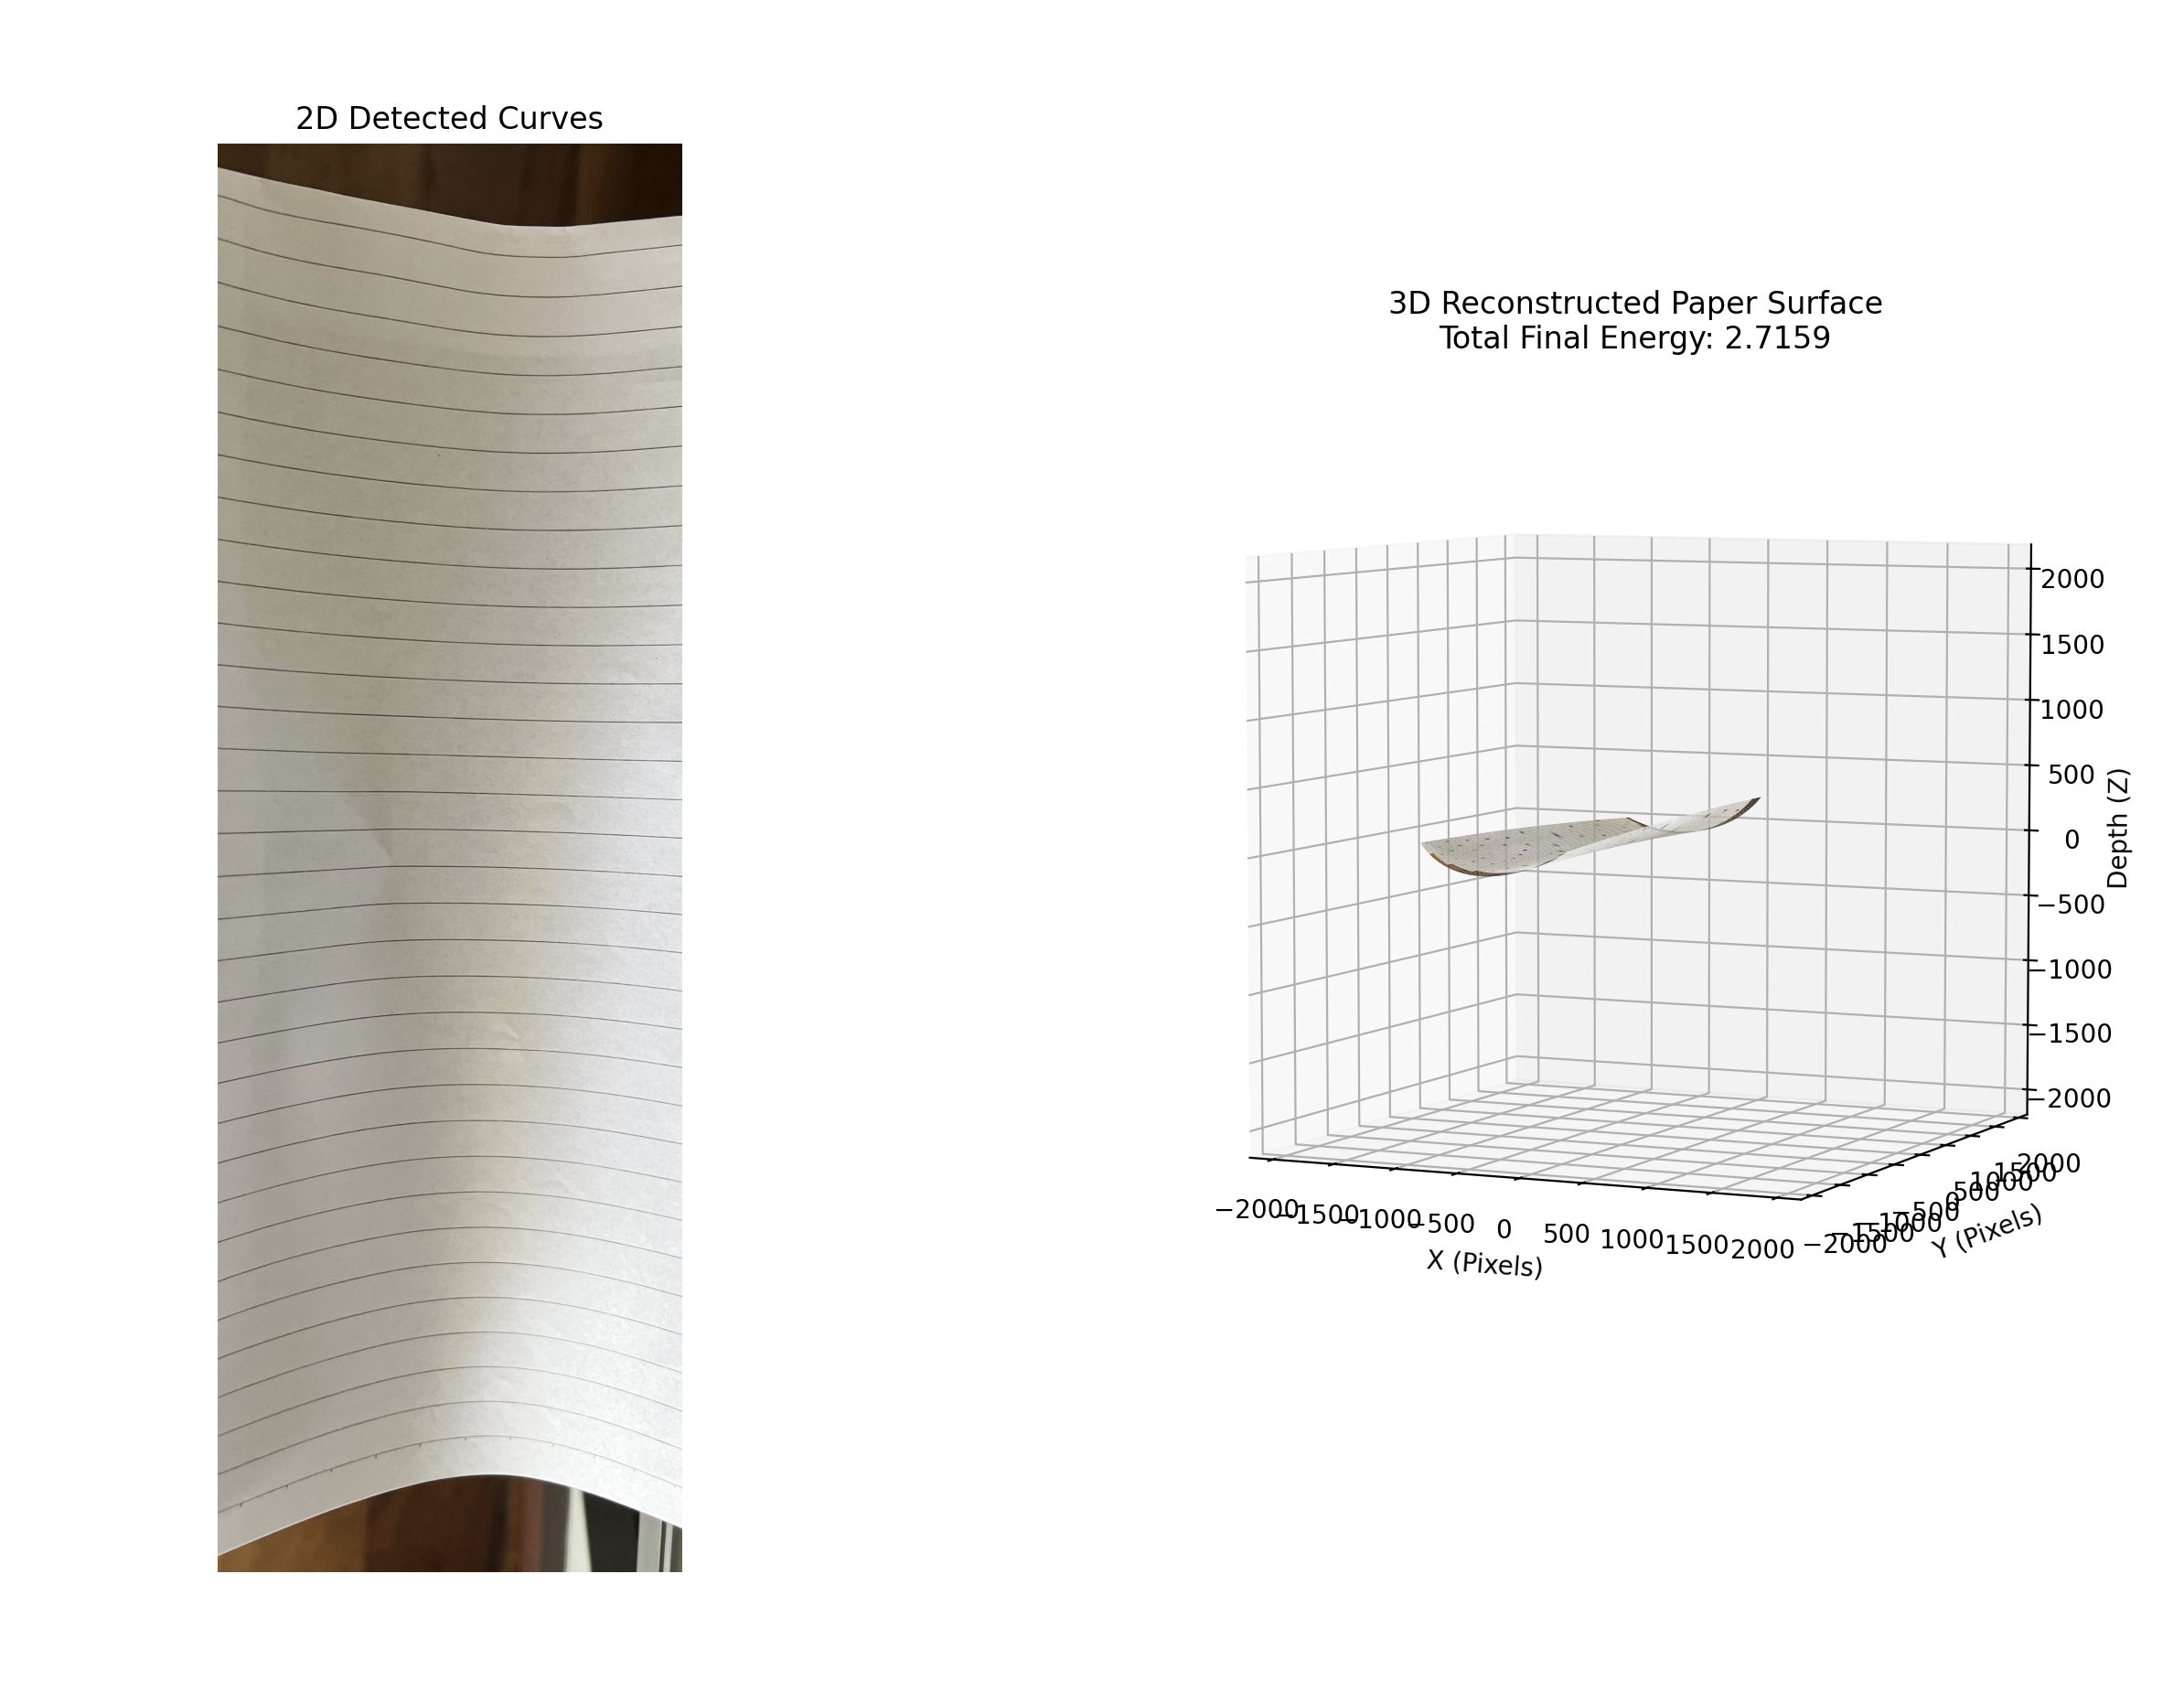
\includegraphics[width=\linewidth,height=0.34\textheight,keepaspectratio]{downcurve.png}
        \caption{Concave deformation (surface curving away from camera).}
        \label{fig:downcurve}
    \end{subfigure}
    \caption{3D surface reconstruction results via energy minimization over extracted rulings, using Adam gradient descent. Left panels show original image,
    while right panels show the reconstructed 3D surface alongside their final minimized energies. (Curve overlay display was disabled for this run.)}
    \label{fig:reconstruction_results}
\end{figure}
Executing \verb|test_gd.py| generates an interactive 3D plot corresponding to Figure \ref{fig:reconstruction_results}, allowing for boundary cropping and manual exclusion of curves exhibiting anomalous high-energy profiles prior to minimization.
\newpage

\section{Why Energy is a Good Metric}\label{sec.isgood}
A natural question is why computing the energy is necessary for a developable surface (such as a piece of paper) that has zero Gaussian curvature everywhere. If the paper is bounded by geodesics (e.g., a perfect rectangle), the problem is trivial. Any geometric disturbance on a developable surface necessarily propagates to at least one boundary. Therefore, information from the boundaries is theoretically sufficient to uniquely construct the surface (up to a global scaling factor, or homothety). The governing PDE can be explicitly derived using Cartan's equations under the constraint $K = 0$. \\~\\
However, if the boundary does not consist of geodesics, boundary data is fundamentally insufficient. Without "outermost" geodesics, curvature information cannot be definitively extrapolated inward. A dense collection of interior horizontal and vertical geodesics is therefore required to uniquely determine the original surface embedding $S$. This requirement extends fully to general non-developable surfaces.\\~\\
Furthermore, PDEs exhibit extreme sensitivity to boundary detection errors. Minor computational inaccuracies can cause the system to become overdetermined or yield non-physical solutions. The energy minimization framework provides a variationally robust alternative that tolerates real-world observational noise. The discrete energy functional $E[\rho] = \sum_\gamma E_\gamma[\rho]$ approximates the continuous integral over the manifold of directional geodesics $G$:
\[
  E = \int_{G_{\text{vert}} \cup G_{\text{hor}}}\int_0^{T} \abs{\ddot \gamma_\rho(t)^T}^2 dt d\gamma_\rho
\]
When minimized, this functional reliably reproduces the original surface geometry across both developable and non-developable embeddings.

\section{Limitations}\label{sec.lim}
A primary limitation of the current implementation stems from the discrete approximation of $\rho$ via the vector $\vect x_0$. While $N$ can be selected to accurately approximate a smooth function, the gradient step $\grad E(\vect x_0)$ yields an updated vector $\vect x_1$ that lacks mathematical guarantees of smoothness. Visualizing the discrete points $(u_i, v_i, x_i)$ mapped from $\vect x_1$ frequently reveals arbitrary jumps and discontinuities. \\~\\
This is precisely why global quadratic fits are employed during gradient descent rather than local bump functions (as detailed in Section \ref{sec.fit}). Applying local fits to discontinuous discrete coordinate sets generates highly irregular, "bumpy" functions that diverge significantly from the true direction of steepest descent. Iterating on these discontinuous intermediate states degrades accuracy and ultimately produces arbitrary surface geometries. \\~\\
The \verb|surface_fit| function conditionally utilizes bump functions but falls back to a global quadratic fit if insufficient points are found in a local bin. By setting \verb|bin_size| to a sufficiently large value, the function is forced into a stabilizing global quadratic fit. Despite providing stability, this fit remains a low-order, crude approximation of $\vect x_1$. \\~\\
Applying a Gaussian blur to the set $\{(u_i, v_i, x_i)\}$ prior to surface fitting could theoretically mitigate localized discontinuities, though this approach has not been rigorously tested and remains constrained by the finite-dimensional approximation. \\~\\
A mathematically rigorous resolution requires formulating the gradient descent directly within a Sobolev space rather than $\R^N$. Instead of vector approximation, gradient descent should act on $E$ as a functional over $C^\infty(Q)$. The gradient $\grad E(\rho)$ must be defined as a $C^k$ function characterizing the Fr\'echet derivative $DE_\rho$. By selecting a Hilbert space $\cal H$, the Riesz representation theorem guarantees the existence of a gradient satisfying $\gen{\grad E(\rho), h}_{\cal H} = DE_\rho (h)$ for all test functions $h \in \cal D$. \\

Using $\cal H = L^2(Q^\circ)$ guarantees an $L^2$ gradient, which may still lack necessary smoothness. Employing the Sobolev space $\cal H = H^m = W^{m, 2}(Q^\circ)$ ensures continuous embeddings into $C^k$ when $m - n/2 > k$. Because $H^m$ is a valid Hilbert space, the iterative algorithm proceeds robustly as $\rho_{n+1} = \rho_n - \eta_n f_n$, where $f_n \in H^m$ satisfies $\gen{f_n, h}_{H^m} = DE_{\rho_n}(h)$ for all $h \in C^\infty(Q)$. \\

Future development priorities include the implementation of this Sobolev gradient descent and the refinement of boundary detection to facilitate accurate surface unrolling and dimension extraction.

\end{document}
